% Figure 1: the system. Compiled on its own by build.sh into build/fig_system.pdf.
\documentclass[tikz,border=0.5pt]{standalone}
\usepackage[T1]{fontenc}
\usepackage[scaled=0.93]{helvet}
\renewcommand{\familydefault}{\sfdefault}
\usepackage{graphicx}
\usetikzlibrary{arrows.meta,calc}

\definecolor{ink}{HTML}{0B0B0B}
\definecolor{ink2}{HTML}{52514E}
\definecolor{rule}{HTML}{C3C2B7}
\definecolor{band}{HTML}{F4F4F1}
\definecolor{gpu}{HTML}{2A78D6}
\definecolor{cloud}{HTML}{EB6834}
\definecolor{cpu}{HTML}{1BAF7A}

% where a part runs: a coloured dot beside ink text (identity never by colour alone)
\newcommand{\chip}[2]{{\color{#1}\raisebox{-0.15ex}{\scalebox{1.6}{$\bullet$}}}\hspace{0.25mm}{\color{ink2}#2}}
\newcommand{\desc}[1]{{\fontsize{5.5}{6.6}\selectfont\color{ink2}#1}}

\begin{document}
\begin{tikzpicture}[x=1mm, y=1mm,
  font=\fontsize{6.1}{7.2}\selectfont\color{ink},
  box/.style={draw=rule, line width=0.4pt, fill=white, rounded corners=1.2mm,
              minimum width=38mm, text width=36.5mm, minimum height=12mm, align=center, inner sep=0.6mm},
  arr/.style={-{Latex[length=1.5mm, width=1.15mm]}, line width=0.55pt, color=ink2},
  lab/.style={font=\fontsize{5.3}{6}\selectfont, text=ink2, inner sep=0.4pt, align=center},
  over/.style={anchor=north west, fill=white, fill opacity=0.86, text opacity=1, inner sep=0.4mm,
               align=left, font=\fontsize{4.5}{5.1}\selectfont\bfseries}]

% ---- the world: what the simulator renders --------------------------------------------------
\node[anchor=south west, inner sep=0] at (0,12.6) {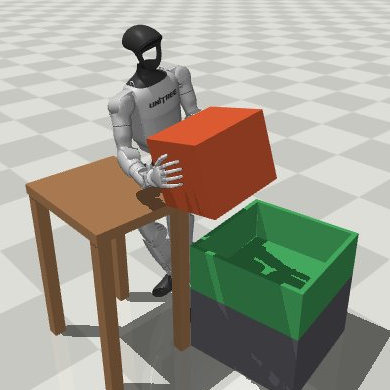
\includegraphics[width=27mm]{img/third_person.png}};
\node[lab, anchor=north west, align=left] at (0,12.2) {scene view, never shown to an agent};
\node[anchor=south west, inner sep=0, align=left] at (0,0.2)
  {\textbf{MuJoCo} \,·\, Unitree G1, 29 DoF\\[0.3mm]\chip{cpu}{\fontsize{5.5}{6.6}\selectfont CPU \,·\, 13\,ms per camera frame}};

\node[anchor=south west, inner sep=0] (h1) at (30,31.2) {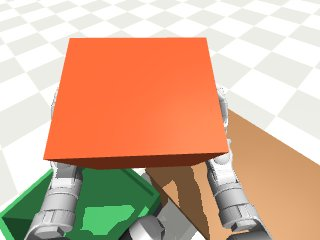
\includegraphics[width=18mm]{img/head_4.png}};
\node[anchor=south west, inner sep=0] (h2) at (30,16.2) {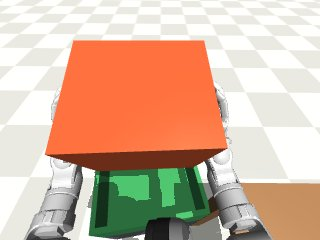
\includegraphics[width=18mm]{img/head_5.png}};
\node[anchor=south west, inner sep=0] (h3) at (30,1.2)  {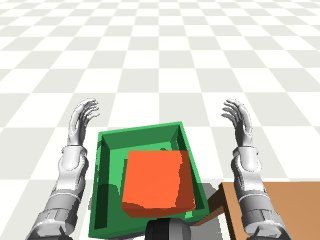
\includegraphics[width=18mm]{img/head_6.png}};
\node[over] at (h1.north west) {bin under left arm\\$\rightarrow$ turn left 45\textdegree};
\node[over] at (h2.north west) {bin under the box\\$\rightarrow$ place};
\node[over] at (h3.north west) {box in the bin\\$\rightarrow$ stop};
\node[anchor=south, font=\fontsize{5.5}{6.3}\selectfont\bfseries, inner sep=0.3mm] at (38,45.0) {head camera: the only sensor};

% ---- bands ------------------------------------------------------------------------------------
\fill[band, rounded corners=1.5mm] (52,23.4) rectangle (187,42.4);
\fill[band, rounded corners=1.5mm] (52,0) rectangle (187,21.2);
\node[anchor=north west, font=\fontsize{5.6}{6.4}\selectfont, text=ink2, inner sep=0] at (54,41.6)
  {\textbf{ACT} \,·\, the deployed loop, on one laptop, no cloud calls};
\node[anchor=north west, font=\fontsize{5.6}{6.4}\selectfont, text=ink2, inner sep=0] at (54,20.4)
  {\textbf{TEACH} \,·\, from one typed sentence, training time only};

% ---- act: student -> safety gate -> controller -> world ----------------------------------------
\node[box] (stu)  at (167,31.4) {\textbf{Student policy}\\\desc{SmolVLM2-500M + LoRA r16}\\\chip{gpu}{\desc{laptop GPU \,·\, 0.3--1.1\,s per decision}}};
\node[box] (gate) at (120,31.4) {\textbf{Safety gate}\\\desc{whitelist, clamps, refusals}\\\chip{cpu}{\desc{CPU}}};
\node[box] (ctl)  at (73,31.4)  {\textbf{Skill controller}\\\desc{IK + joint PD; Unitree RL legs}\\\chip{cpu}{\desc{CPU \,·\, 0.03\,ms per 50\,Hz tick}}};

\draw[arr] (48.3,43.9) -- (167,43.9) -- (stu.north);
\node[lab, anchor=south] at (108,44.1) {head frame + instruction + last skill's feedback};
\draw[arr] (stu.west) -- node[lab, above=0.3mm] {skill call} (gate.east);
\draw[arr] (gate.west) -- node[lab, above=0.3mm] {allowed} (ctl.east);
\draw[arr] (ctl.west) -- (48.4,31.4);

% ---- teach: world -> validator -> Argon -> fine-tune -> student --------------------------------
\node[box] (val) at (73,11)  {\textbf{Validator}\\\desc{ground truth $\rightarrow$ verdict in words}\\\chip{cpu}{\desc{CPU}}};
\node[box] (arg) at (120,11) {\textbf{Argon teacher}\\\desc{writes the task, diagnoses, demonstrates}\\\chip{cloud}{\desc{cloud \,·\, 8.1\,s per call}}};
\node[box] (ft)  at (167,11) {\textbf{LoRA fine-tune}\\\desc{accepted teacher steps only}\\\chip{gpu}{\desc{laptop GPU \,·\, 21\,min per fine-tune}}};

\draw[arr] (48.4,11) -- (val.west);
\draw[arr] (val.east) -- node[lab, above=0.3mm] {failure} (arg.west);
\draw[arr] (arg.east) -- node[lab, above=0.3mm] {accepted} (ft.west);
\draw[arr] (ft.north) -- node[lab, right=0.6mm] {new checkpoint} (stu.south);
\draw[arr, dash pattern=on 1.4pt off 1pt] (arg.south) -- (120,2.0) -- (48.6,2.0);
\node[lab, anchor=south] at (86,2.2) {Argon drives the robot itself: same camera, same skills};
\end{tikzpicture}
\end{document}
